\chapter{Resultados}
\label{chap:resultados}

\drop{E}{n} este capítulo se introducirán los recursos y costes empleados por GrayAR. Se presentarán estadísticas del proyecto y algunas medidas de rendimiento que se han calculado junto a sus
resultados. Respecto al apartado de costes, se hará una estimación de éstos de acuerdo a las condiciones de mercado actuales.

Para finalizar, se muestra el funcionamiento del sistema desarrollado dentro del \textit{Proyecto ARgos} mediante varios casos de usos.  

\section{Estadísticas del Repositorio}

La Tabla~\ref{tab:number_of_lines} muestra el número de líneas de código de GrayAR. Se han omitido
sin embargo las líneas de código pertenecientes a las herramientas externas desarrolladas y a los
\textit{scripts} ARS creados, los cuales sumarían en torno a 2000 líneas más de código. Para
contabilizar dichas líneas, se ha empleado la aplicación \textbf{\textit{cloc}}.

\begin{table}[h]
  \centering
  \begin{tabular}{|l|r|r|r|r|}
    \hline
    \textbf{Lenguaje} & \textbf{Archivos} & \textbf{Espacios en blanco} & \textbf{Comentarios} & \textbf{Líneas de código} \\
    \hline
    \textit{C++} & 30 & 942 & 472 & 3480 \\
    \hline
    \textit{Cabeceras C/C++} & 34 & 601 & 1546 & 1392 \\
    \hline
    \textit{GLSL} & 12 & 0 & 0 & 99 \\
    \hline
    \textit{make} & 2 & 29 & 0 & 93 \\
    \hline
    \textbf{Total:} & \textbf{66} & \textbf{1572} & \textbf{2018} & \textbf{4965} \\
    \hline
  \end{tabular}
  \caption{Número de líneas del código fuente de GrayAR.}
  \label{tab:number_of_lines}
\end{table}

\section{Recursos y costes}
El desarrollo del presente Trabajo de Fin de Grado abarcó desde el día 18 de Noviembre de 2013, hasta
el 25 de Noviembre de 2014, aproximadamente. En la contabilización no se ha tenido en cuenta el tiempo dedicado a la documetación de la presente memoría, ni los periodos vacacionales, por lo que el tiempo total de desarrollo y pruebas ha supuesto una duración de 43 semanas. Con una dedicación media de 7 horas diarias (5 días a la semana), se traduce en 1505 horas de trabajo. 

Se ha supuesto un precio de \textit{\EUR{30}/hora} tomando como referencia la media de cobro actual
de mercado en este sector~\footnote{Información obtenida de
  \url{https://freelance.infojobs.net/freelancers/programador/informatica}.}.

La Tabla~\ref{tab:costs} muestra un desglose de gastos aproximados para el desarrollo de
GraAR. La tabla incluye todo el hardware necesario para la puesta en marcha del sistema, así como
el sueldo del programador calculado teniendo en cuenta lo anterior. Se muestra también el coste
en total del proyecto.

El coste obtenido es meramente informativo, ya que a la hora de calcular un presupuesto se deben de
tener en cuenta otros muchos factores.

\begin{table}[h]
  \centering
  \begin{tabular}{|l|r|r|}
    \hline
    \textbf{Recurso} & \textbf{Cantidad} & \textbf{Coste} \\
    \hline
    Sueldo programador (1505 horas) & 1 & \EUR{45.150} \\
    \hline
    Computador de trabajo & 1 & \EUR{499} \\
    \hline
    Raspberry Pi (Modelo B) & 1 & \EUR{40} \\
    \hline
    Cámara Raspberry Pi & 1 & \EUR{24,95} \\
    \hline
    Proyector Optoma PK320 & 1 & \EUR{325} \\
    \hline
    MicroSDHC Trascend 32GB & 1 & \EUR{14,75} \\
    \hline
    Altavoz WaveShare LM386 & 1 & \EUR{10} \\
    \hline
    Webcam Logitech HD C270 & 1 & \EUR{26} \\
    \hline
    \textbf{Total} & & \EUR{46.089,7} \\
    \hline
  \end{tabular}
  \caption{Desglose de costes de GrayAR.}
  \label{tab:costs}
\end{table}


\section{Profiling}

\subsection{Rendimiento de cámaras utilizadas}

\subsection{Rendimiento del sistema a distintas resoluciones}
\subsection{Velocidad y tasa de aciertos de los descriptores de imágenes}
\subsection{Histórico de Percepciones}
\subsection{Rendimiento general del sistema en cada una de las iteraciones}



\section{Prototipo hardware construido}
El prototipo construido emplea una cámara de bajo coste como entrada al módulo de visión por computador y un cañón de proyección portátil para mostrar información visual, directamente alineada sobre el documento del mundo físico. La ejecución del software del sistema la realiza la unidad Raspberry Pi, que se encarga de tomar como entrada las imágenes obtenidas por la cámara y generar la salida para el cañón de proyección. También se ha incluido un amplificador con altavoz incorporado para la reprodución de mensajes y alertas del sistema.

Para obtener un conjunto compacto y reducido, se acopla la Raspberry Pi sobre el proyector y la raspiCam junto a la lente. En la figura ~\ref{fig:ARgos_hardware} se muestran por separado los componentes hardware empleados, así como su disposición final en el prototipo.

\begin{figure}
  \begin{center}
    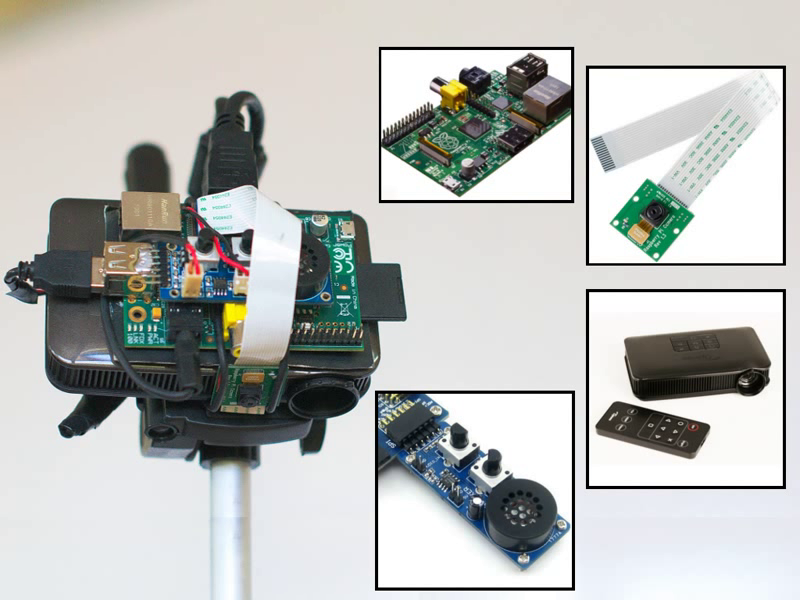
\includegraphics[width=1.0\textwidth]{ARgos_hardware.png}
    \caption{Hardware de ARgos.}
    \label{fig:ARgos_hardware}
  \end{center}
\end{figure}

Finalmente, el sistema se monta sobre un trípode y se coloca en dirección a la mesa. Siendo la colocación final de uso la que se aprecia en la figura \ref{fig:ARgos_user} 

\begin{figure}
  \begin{center}
    \includegraphics[width=1.0\textwidth]{argos_user.png}
    \caption{Disposición del prototipo en un escenario real}
    \label{fig:ARgos_user}
  \end{center}
\end{figure}


\section{Uso del sistema}

A continuación, se introducirá un caso de uso concreto del sistema \textit{ARgos}, mediante imágenes del funcionamiento real del prototipo. 

\subsection{Prerrequisitos}
Previamente, el usuario ha calibrado el sistema utilizando la herramienta que se proporciona, y de la que obtiene una serie de ficheros, que deben ser copiados en el cliente y el servidor. En estos ficheros se encuentran los parámetros instrinsecos de la cámara y el proyector, asi como las matrices de transformación entre el sistema de coordenadas de la cámara y el del proyector.

Asimismo, el usuario ha proporcionado una imagen de cada uno de los documentos posibles a identificar por el sistema, y las acciones a realizar o representar en ellos. Esta configuración se realiza por medio de los \textit{scripts} implementados en \textit{BelfegAR}.
 
\subsection{Carga del sistema}
Tras el encendido del prototipo,  Durante la carga del sistema, el registro de eventos muestra por la salida especificada los sucesos correspondientes al cliente y el servidor durante esa etapa (véase Figura~\ref{fig:Client_init} y
Figura~\ref{fig:Server_init}, respectivamente). Para el cliente (y detallando el registro correspondiente a ARgos), el registro muestra que la conexión con el servidor se ha realizado
correctamente, la inicialización del contexto OpenGL ES y la carga de imágenes que se usarán más tarde por el sistema. Para el caso del servidor, el registro muestra la carga en memoria de los
\textit{scripts} y la IP y el puerto donde está escuchando conexiones de clientes.

\begin{figure}[!h]
  \begin{center}
    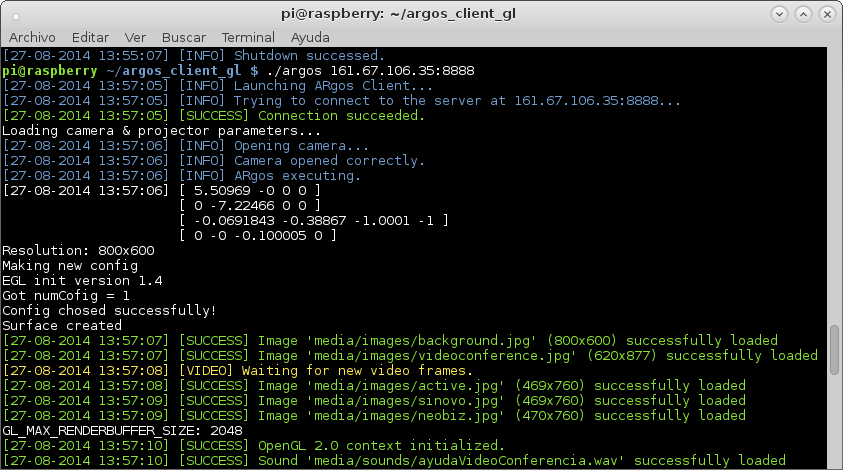
\includegraphics[width=1.0\textwidth]{Client_init.png}
    \caption{Inicialización del cliente.}
    \label{fig:Client_init}
  \end{center}
\end{figure}

\begin{figure}[!h]
  \begin{center}
    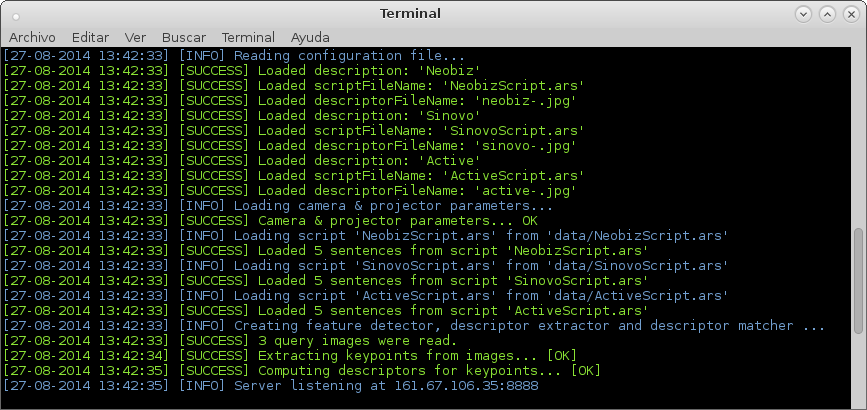
\includegraphics[width=1.0\textwidth]{Server_init.png}
    \caption{Inicialización del servidor.}
    \label{fig:Server_init}
  \end{center}
\end{figure}

Arrancado el sistema, el proyector muestra una imagen cargada desde disco por \textit{ARgos} con información sobre un supuesto usuario ficticio (véase Figura~\ref{fig:ARgos_intro}).

\begin{figure}
  \begin{center}
    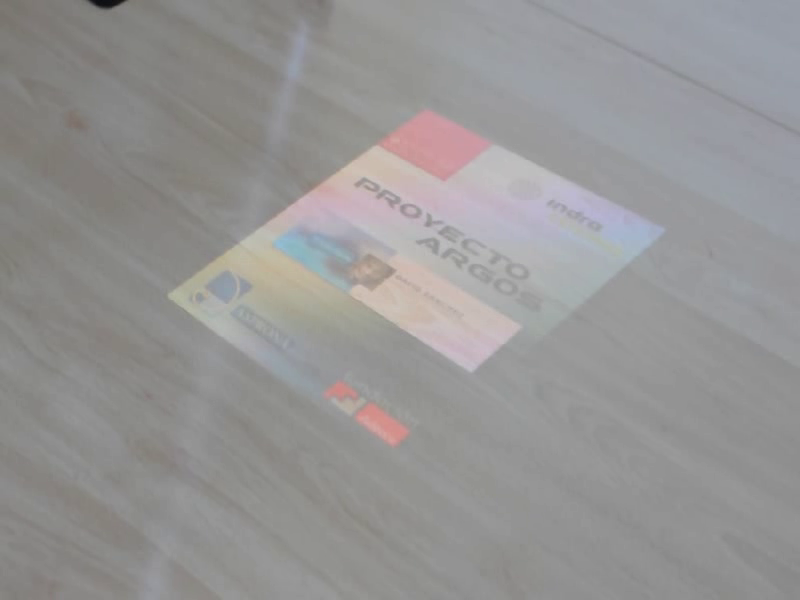
\includegraphics[width=0.9\textwidth]{ARgos_intro.png}
    \caption{Arranque de ARgos.}
    \label{fig:ARgos_intro}
  \end{center}
\end{figure}


\subsection{Bucle principal}

Al finalizar la introducción, el sistema avanza hacia el próximo estado entrando en el bucle principal de detección de documentos, delegación de tareas y renderizado. Este estado es fácilmente reconocible por proyectar las cuatro esquinas que delimitan el área de trabajo sobre la superficie (véase Figura~\ref{fig:ARgos_waiting}).

\begin{figure}
  \begin{center}
    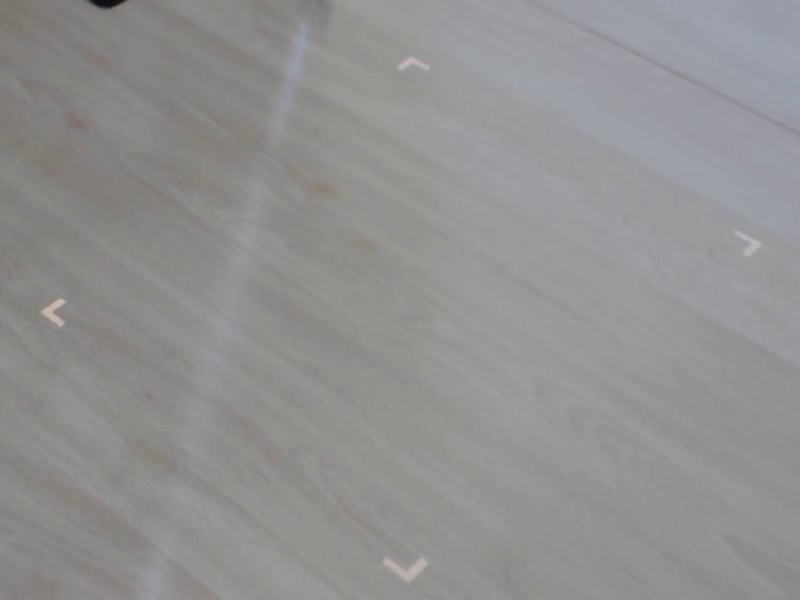
\includegraphics[width=0.9\textwidth]{ARgos_waiting.png}
    \caption{ARgos esperando por documentos.}
    \label{fig:ARgos_waiting}
  \end{center}
\end{figure}


A partir de este momento, el usuario puede empezar a colocar los documentos sobre la superficie de trabajo. Tras situar el primer documento, el sistema detecta la hoja de papel, calcula su posición en el espacio 3D e identifica el documento por su contenido. Con esta información, \textit{BelfegAR} renderiza varios componentes gráficos, como zonas de resaltado, correspondientes a ese documento. Para este caso concreto, se presentan varios botones que el usuario puede pulsar e iniciar un vídeo que traduce a lengua de signos el documento. (véase Figura~\ref{fig:ARgos_facture1}).

\begin{figure}
  \begin{center}
    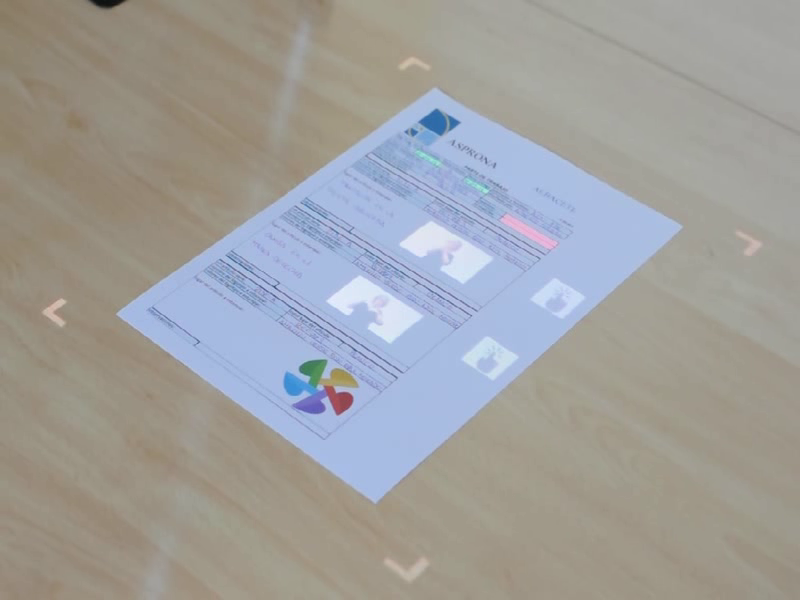
\includegraphics[width=0.9\textwidth]{ARgos_facture1.png}
    \caption{Primer documento detectado y componentes gráficos desplegados.}
    \label{fig:ARgos_facture1}
  \end{center}
\end{figure}

Después, el usuario coloca un segundo documento. Para este caso, el sistema renderiza otros componentes gráficos basados en el contexto del formulario detectado (véase Figura~\ref{fig:ARgos_facture2}). Además, se presentan varios botones que el usuario puede pulsar para obtener información adicional de forma ampliada al darle la vuelta al documento, y utilizar la parte trasera como «pantalla de proyección». (véase Figura~\ref{fig:ARgos_facture2_1}).

\begin{figure}
  \begin{center}
    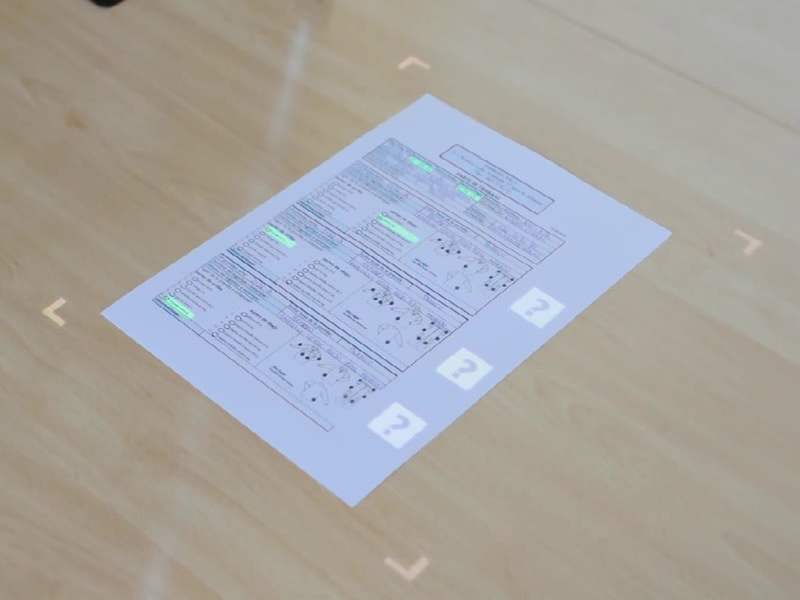
\includegraphics[width=0.9\textwidth]{ARgos_facture2.png}
    \caption{Segundo documento detectado y componentes gráficos desplegados.}
    \label{fig:ARgos_facture2}
  \end{center}
\end{figure}

\begin{figure}
  \begin{center}
    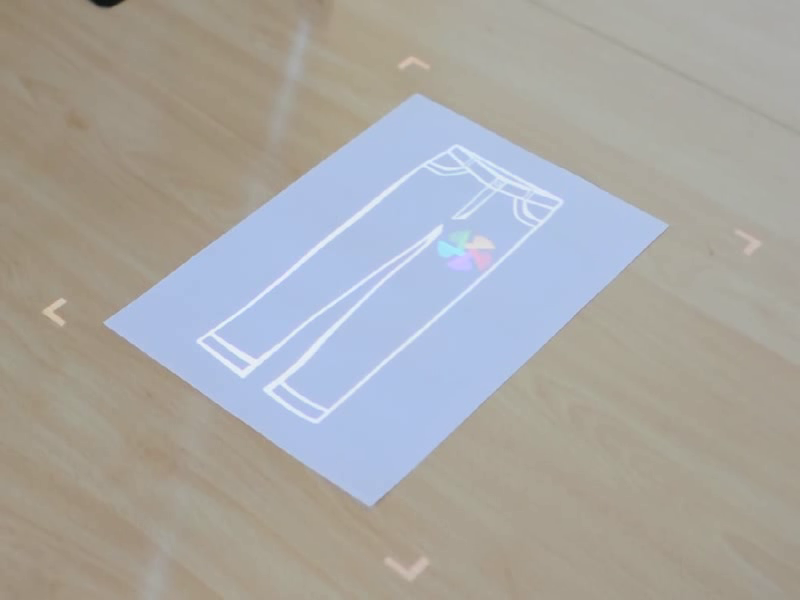
\includegraphics[width=0.9\textwidth]{ARgos_facture2_1.png}
    \caption{Segundo documento al pulsar el botón de interacción.}
    \label{fig:ARgos_facture2_1}
  \end{center}
\end{figure}


Entre las acciones a realizar en el tercer documento, está definida la posibilidad de realizar una videollamada. Tras la pulsación del botón correspondiente y volteando nuevamente el documento (véase Figura~\ref{fig:ARgos_facture3}). 

La Figura~\ref{fig:ARgos_videostream2} muestra como se han empezado a recibir fotogramas del servidor y son renderizados sobre el propio documento junto a una imagen de fondo.

\begin{figure}
  \begin{center}
    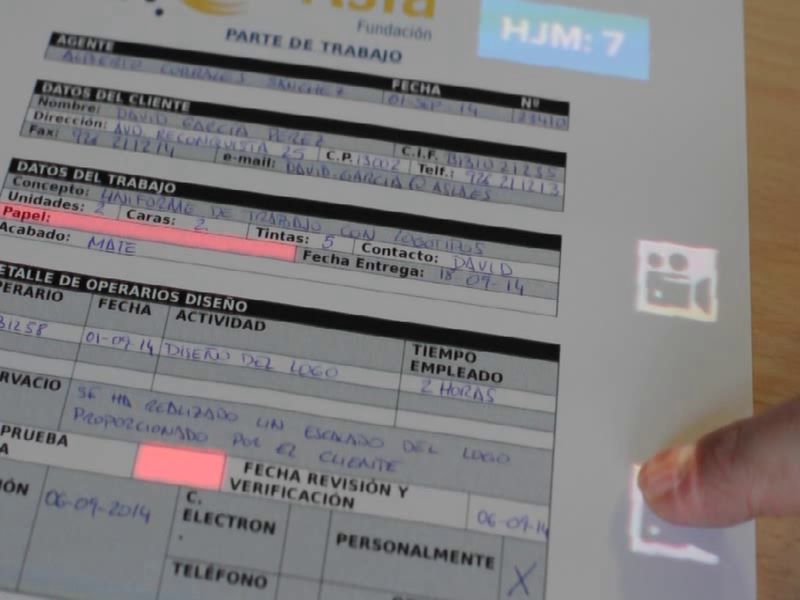
\includegraphics[width=0.9\textwidth]{pulsacion.png}
    \caption{Tercer documento detectado y componentes gráficos desplegados.}
    \label{fig:ARgos_facture3}
  \end{center}
\end{figure}

\begin{figure}
  \begin{center}
    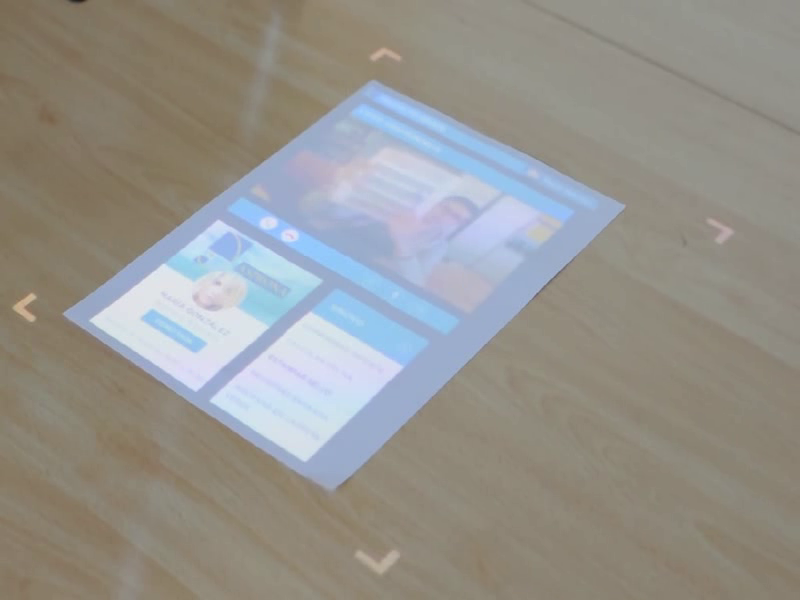
\includegraphics[width=0.9\textwidth]{ARgos_videostream2.png}
    \caption{Videollamada iniciada sobre la superficie del documento.}
    \label{fig:ARgos_videostream2}
  \end{center}
\end{figure}

Durante toda la ejecución del sistema se realiza un registro de los eventos ocurridos. La Figura~\ref{fig:Client_loop} y la Figura~\ref{fig:Server_listening} muestran respectivamente los registros de eventos del cliente y
del servidor mientras se ejecuta el bucle principal del sistema. En ellos se puede apreciar las matrices de transformación de cada documento detectado o la comunicación realizada entre cliente y servidor.

\begin{figure}
  \begin{center}
    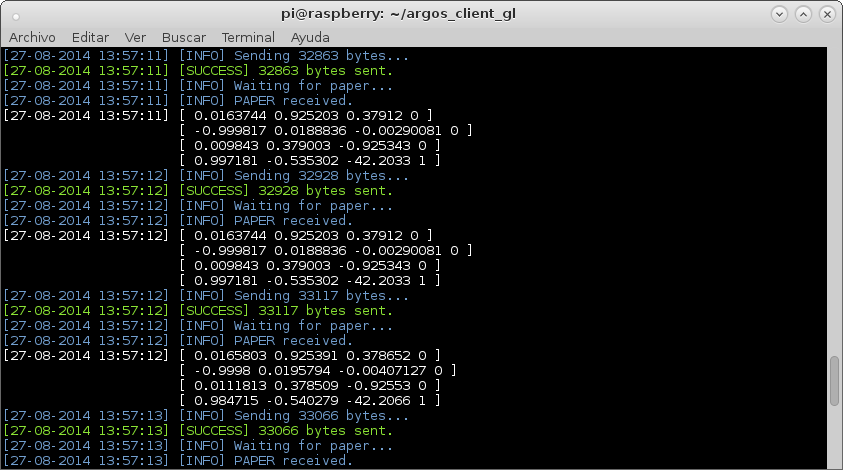
\includegraphics[width=1.0\textwidth]{Client_loop.png}
    \caption{Registro de eventos del cliente mientras se ejecuta el bucle principal del sistema.}
    \label{fig:Client_loop}
  \end{center}
\end{figure}

\begin{figure}
  \begin{center}
    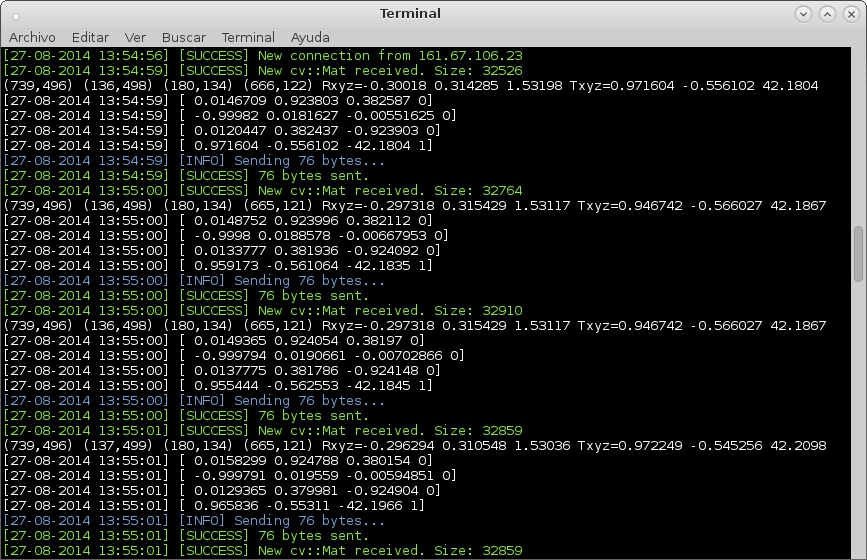
\includegraphics[width=1.0\textwidth]{Server_listening.png}
    \caption{Registro de eventos del servidor mientras se ejecuta el bucle principal del sistema.}
    \label{fig:Server_listening}
  \end{center}
\end{figure}

%Finalmente, la Figura~\ref{fig:Client_release} muestra el cierre del cliente de manera limpia liberando la memoria del sistema y cerrando los subsistemas adecuados.

%\begin{figure}[!h]
%  \begin{center}
%    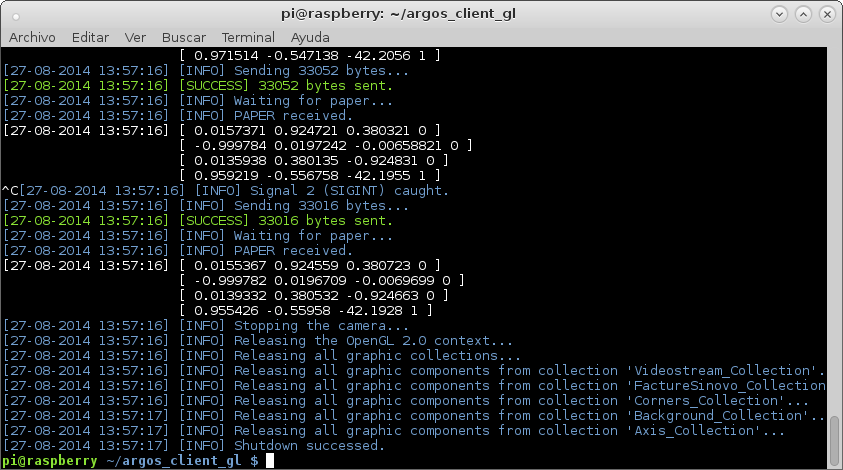
\includegraphics[width=1.0\textwidth]{Client_release.png}
%    \caption{Cierre de sistemas y liberación de la memoria del cliente.}
%    \label{fig:Client_release}
%  \end{center}
%\end{figure}













